\begin{IEEEbiography}
[{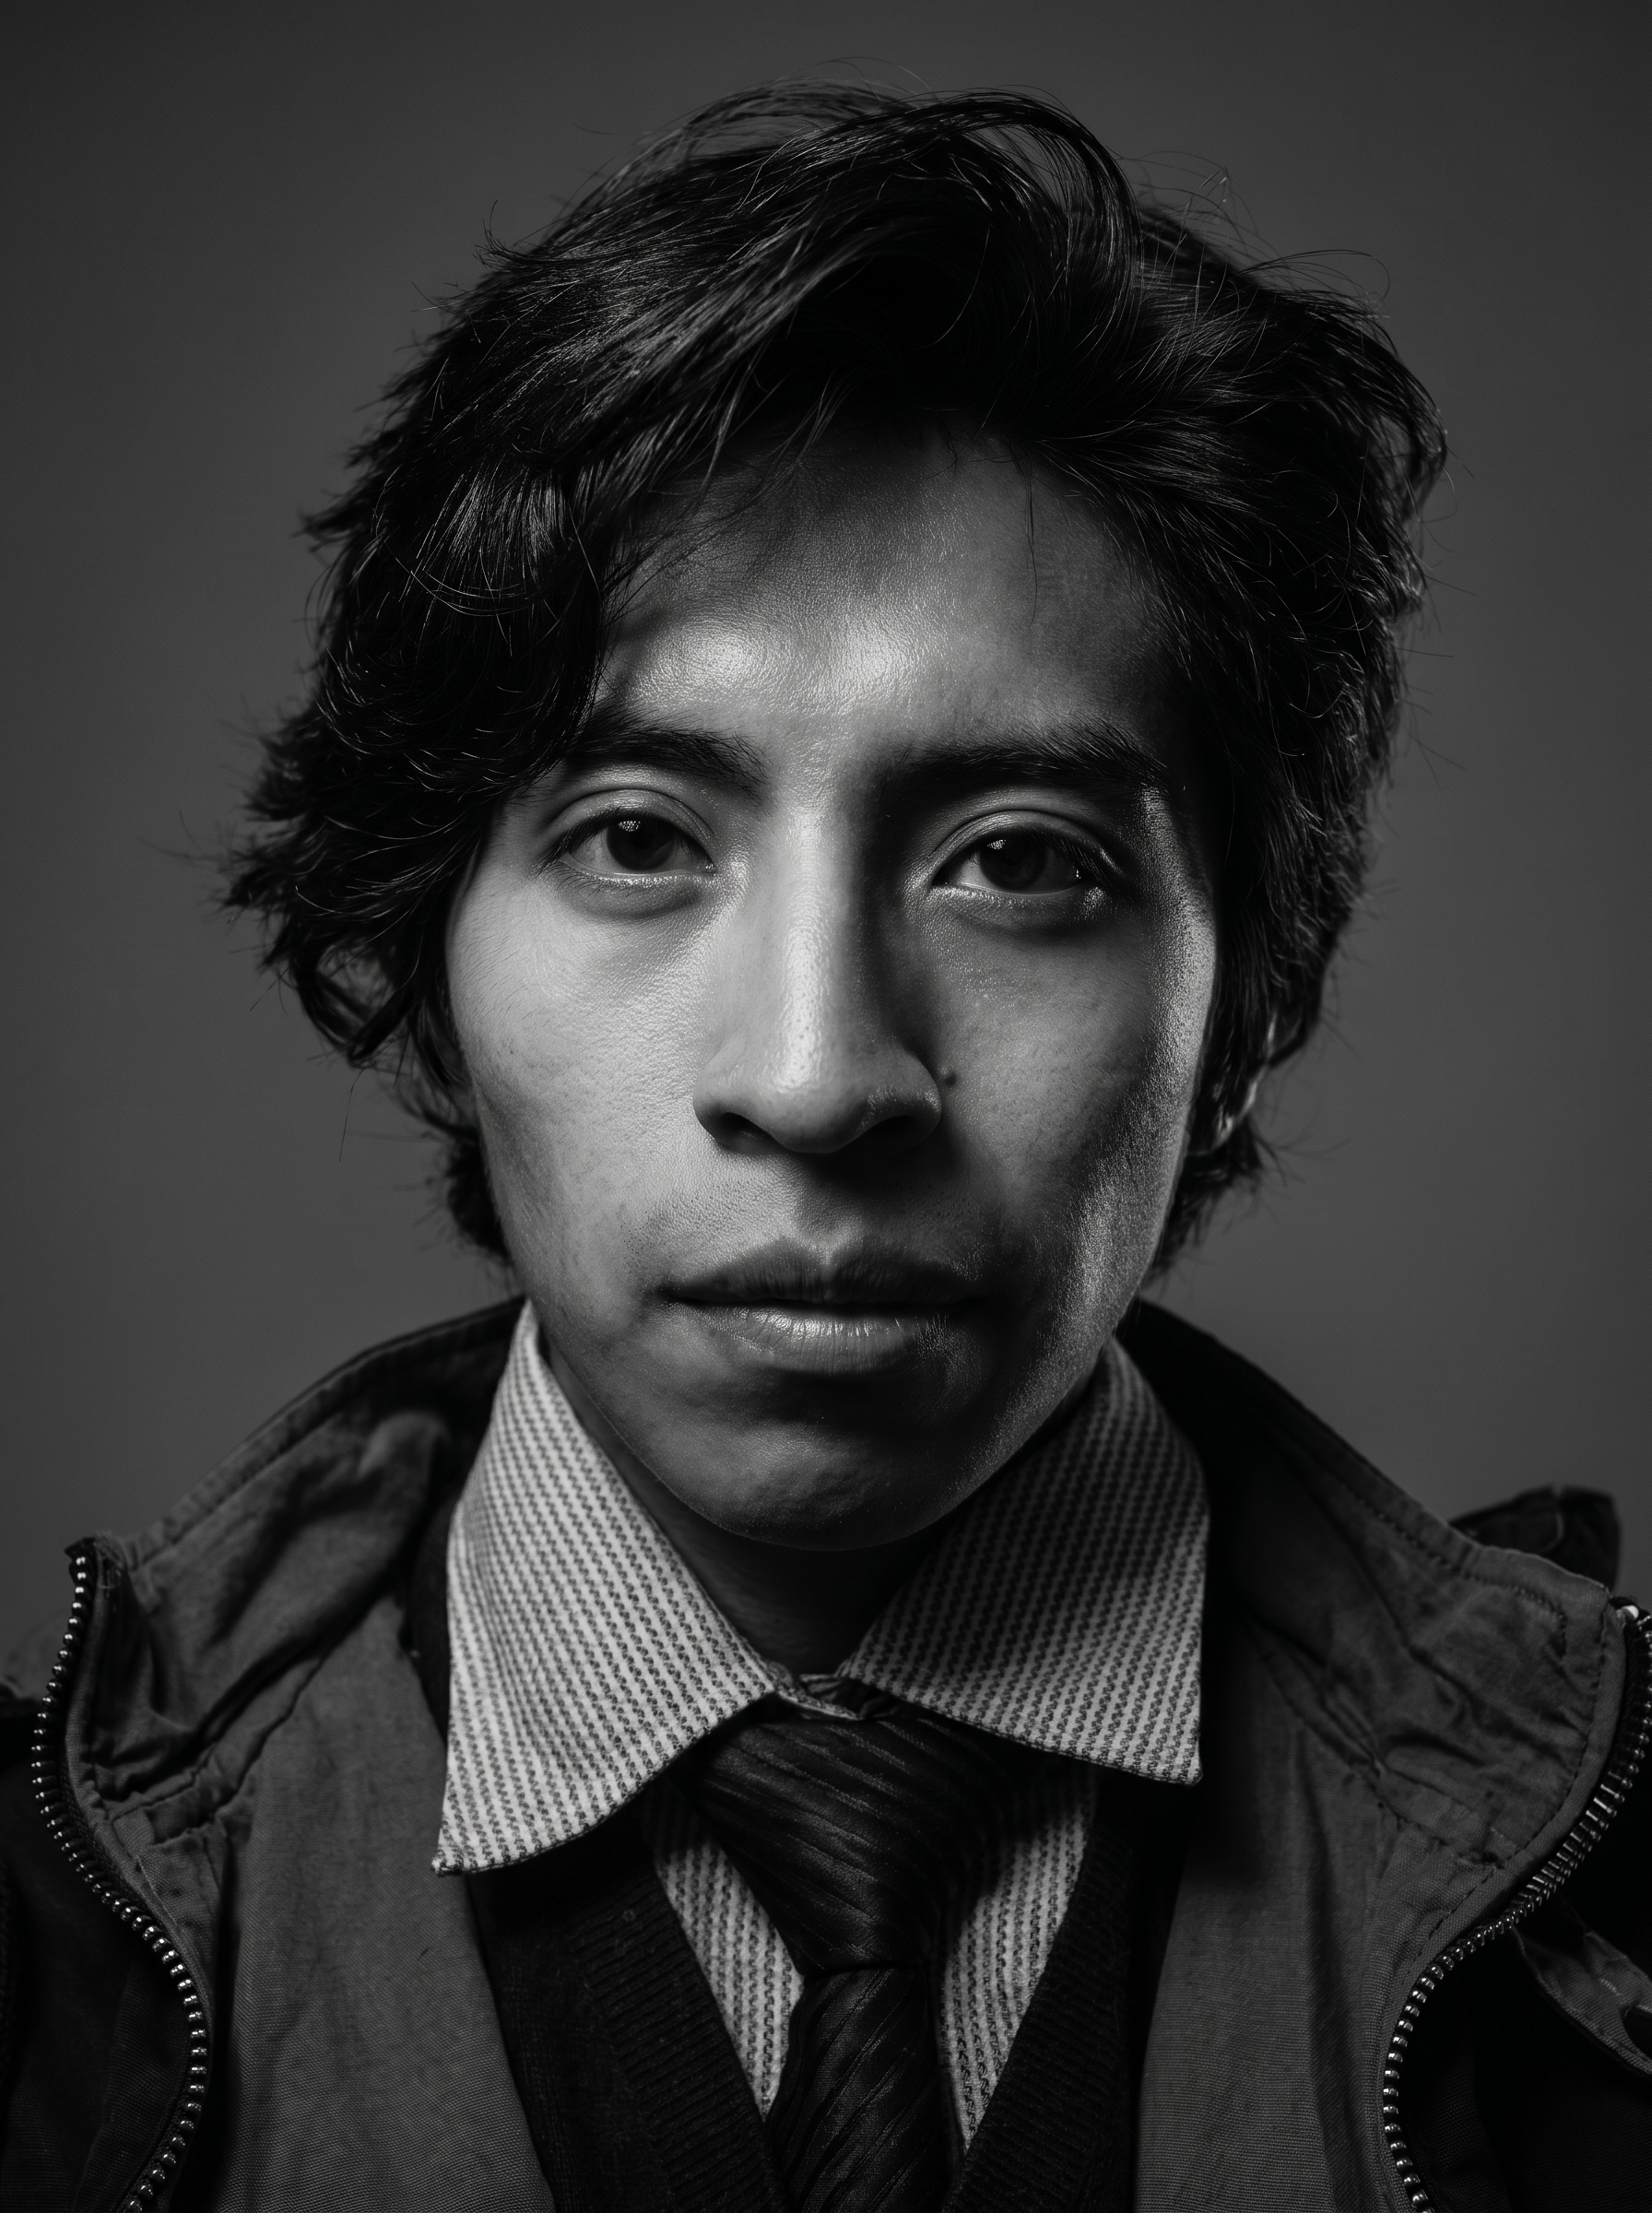
\includegraphics[width=1in,height=1.25in,clip,keepaspectratio]{images/Byron.jpeg}}]{Byron Paul Condolo Narvaez}
es estudiante de la carrera de Computación en la Facultad de Ingeniería y Ciencias Aplicadas de la Universidad Central del Ecuador (UCE). Sus intereses de investigación se centran en el área de sistemas distribuidos, simulación basada en agentes y ciberseguridad corporativa.
\end{IEEEbiography}

\begin{IEEEbiography}
[{
\includegraphics[width=1in,height=1.25in,clip,keepaspectratio]{images/Kelly.jpeg}}]{Kelly Denisse Ledesma Aguilar}
es estudiante de la carrera de Computación en la Facultad de Ingeniería y Ciencias Aplicadas de la Universidad Central del Ecuador (UCE). Sus áreas de interés académico incluyen la seguridad de la información, análisis de vulnerabilidades y la modelación computacional de redes complejas.
\end{IEEEbiography}

\begin{IEEEbiography}
[{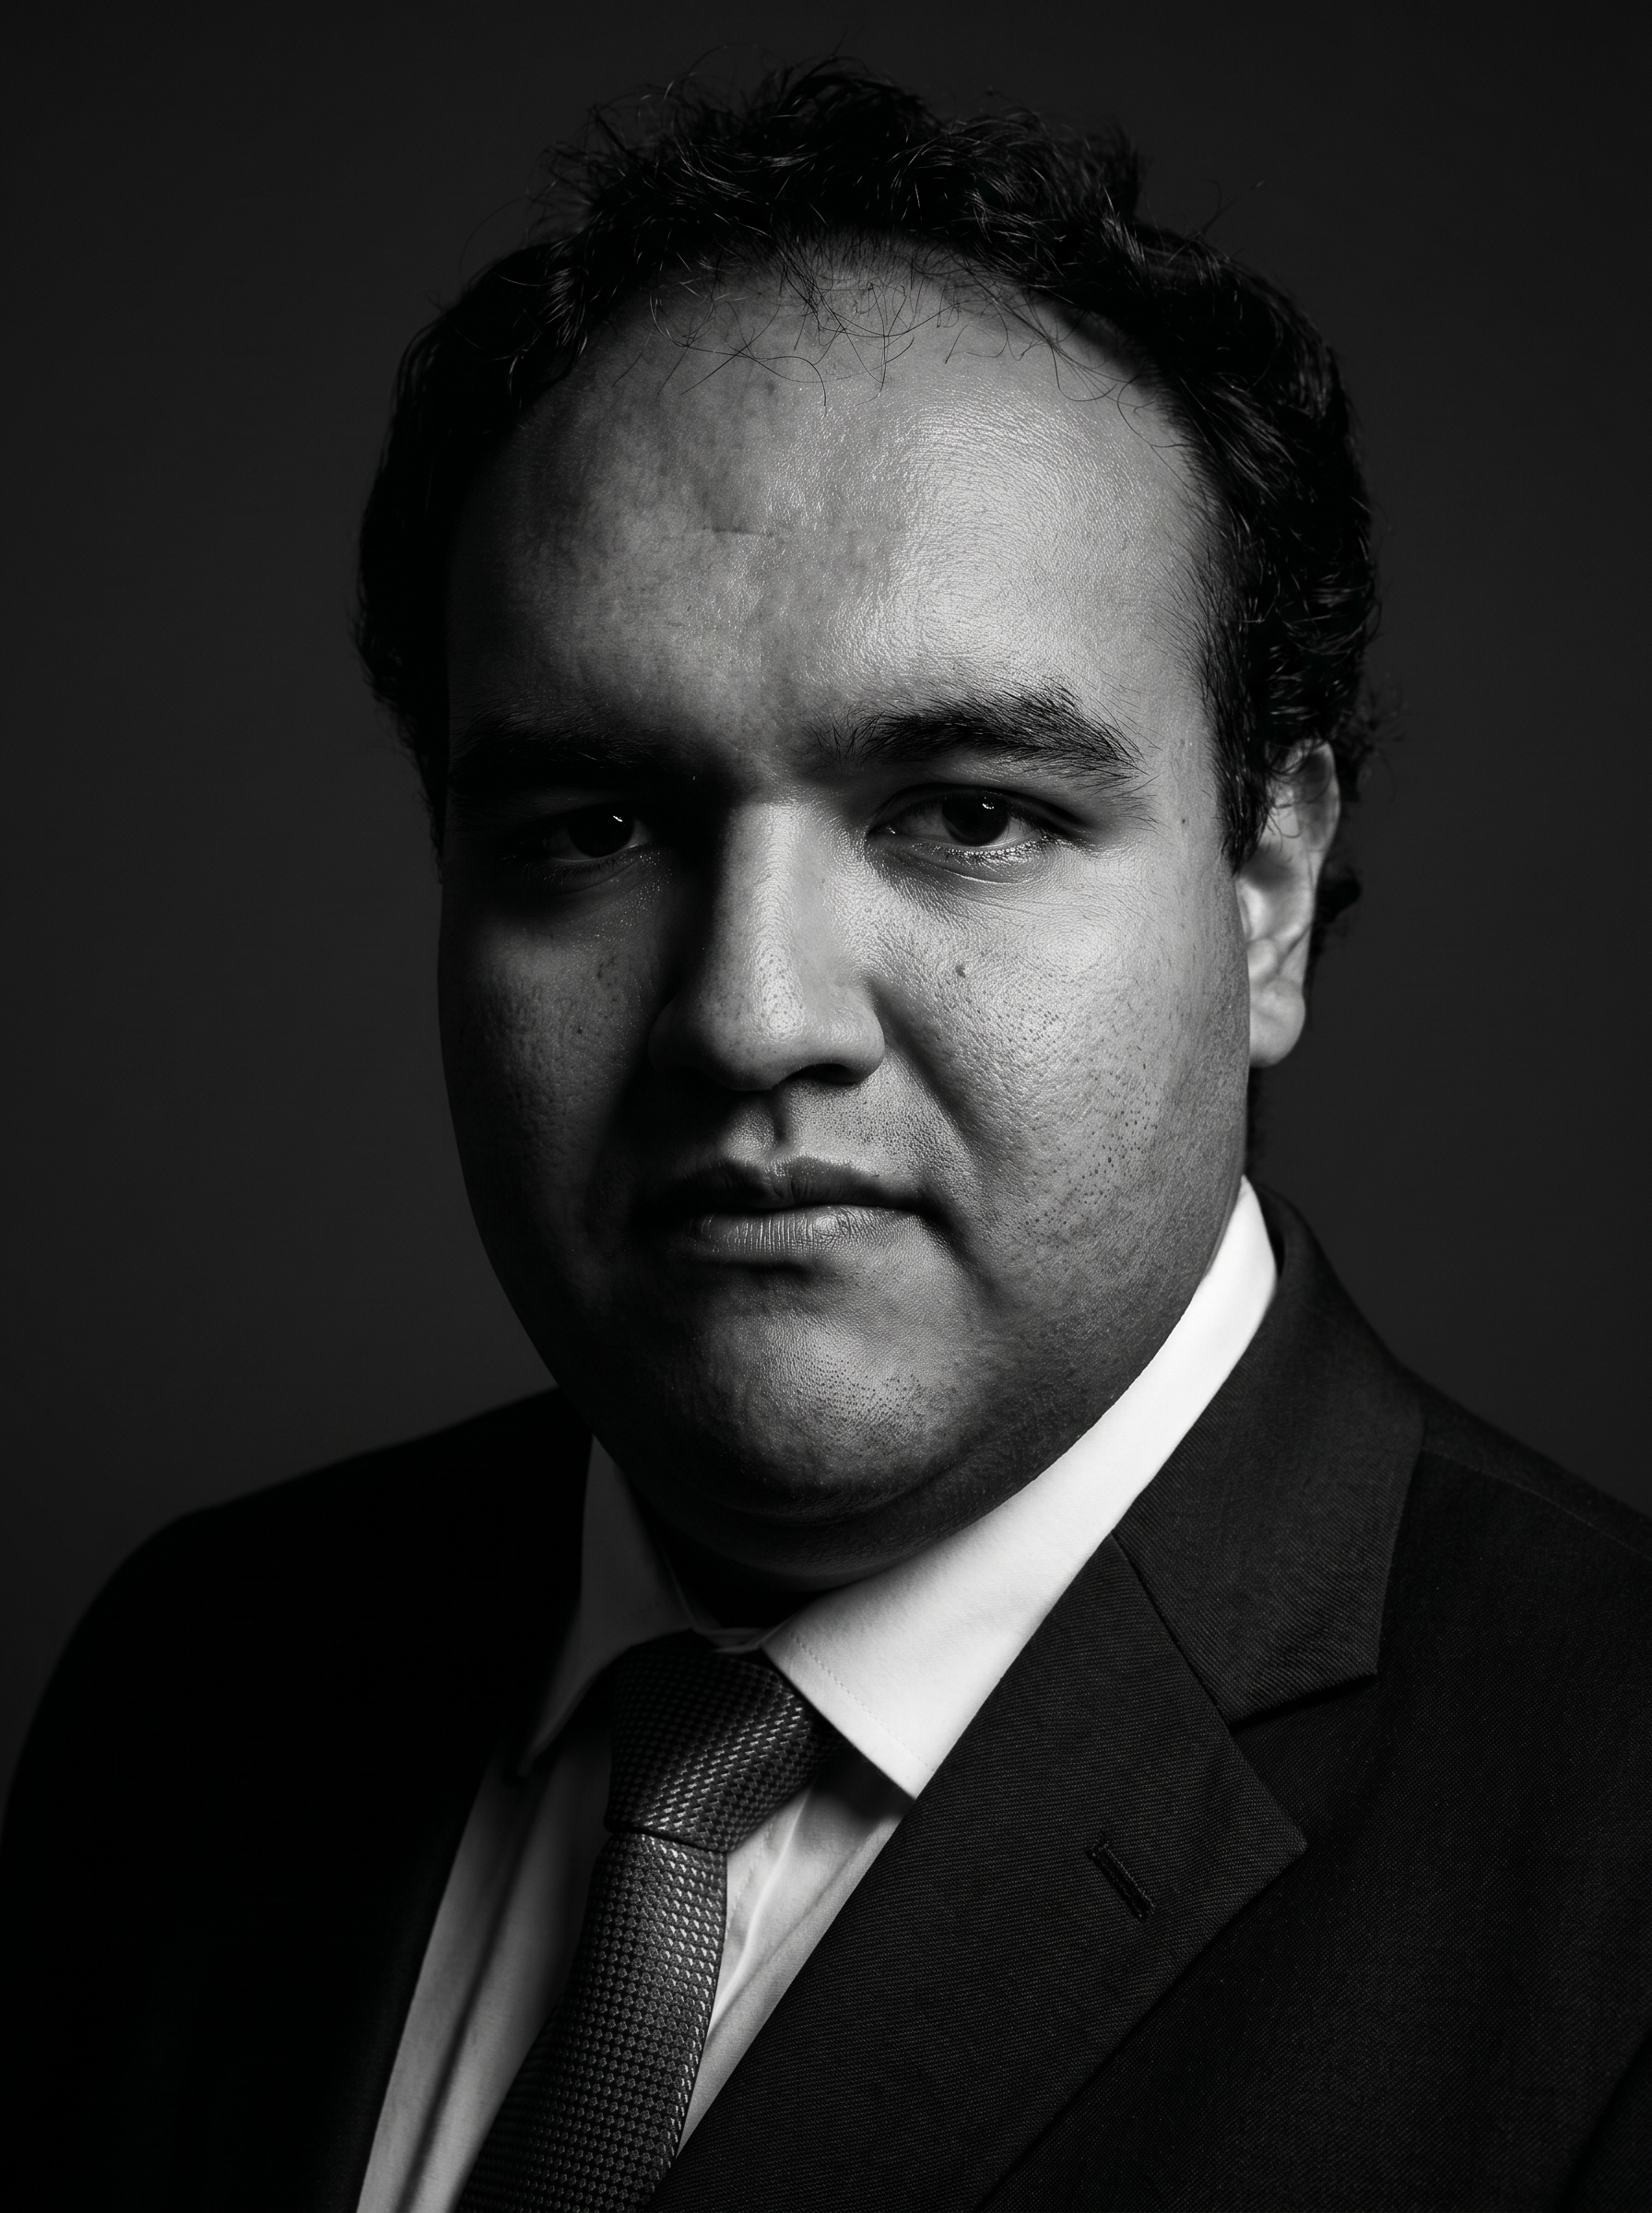
\includegraphics[width=1in,height=1.25in,clip,keepaspectratio]{images/Bryan.jpeg}}]{Bryan Eduardo Loya Cadena}
es estudiante de la carrera de Computación en la Facultad de Ingeniería y Ciencias Aplicadas de la Universidad Central del Ecuador (UCE). Actualmente se enfoca en el estudio de sistemas colaborativos, simulación con sistemas multiagente y el diseño de políticas reactivas ante incidentes informáticos.
\end{IEEEbiography}

\begin{IEEEbiography}
[{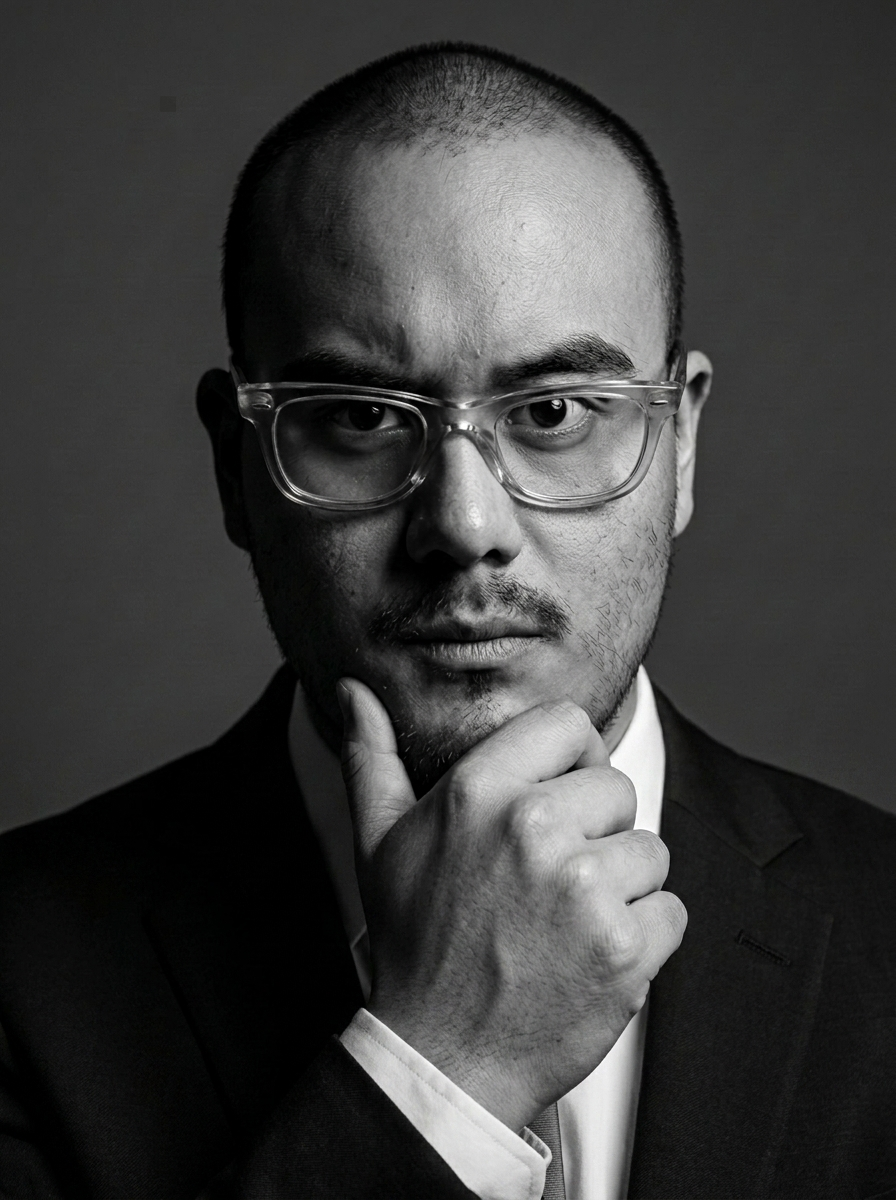
\includegraphics[width=1in,height=1.25in,clip,keepaspectratio]{images/Dennis.jpeg}}]{Dennis Adrian Trujillo Vistin}
es estudiante de la carrera de Computación en la Facultad de Ingeniería y Ciencias Aplicadas de la Universidad Central del Ecuador (UCE). Sus intereses de investigación abarcan el análisis forense de malware, simulación basada en GIS en la plataforma GAMA y la administración de seguridad en redes LAN académicas.
\end{IEEEbiography}
